%% LyX 1.6.2 created this file.  For more info, see http://www.lyx.org/.
%% Do not edit unless you really know what you are doing.
\documentclass[english]{IEEEtran}
\usepackage[T1]{fontenc}
\usepackage[latin9]{inputenc}
\usepackage{babel}

\usepackage{float}
\usepackage{textcomp}
\usepackage{amsthm}
\usepackage{amsmath}
\usepackage{graphicx}
\usepackage[unicode=true, pdfusetitle,
 bookmarks=true,bookmarksnumbered=false,bookmarksopen=false,
 breaklinks=false,pdfborder={0 0 1},backref=false,colorlinks=false]
 {hyperref}

\makeatletter

%%%%%%%%%%%%%%%%%%%%%%%%%%%%%% LyX specific LaTeX commands.
\newcommand{\noun}[1]{\textsc{#1}}
%% Because html converters don't know tabularnewline
\providecommand{\tabularnewline}{\\}
\floatstyle{ruled}
\newfloat{algorithm}{tbp}{loa}
\floatname{algorithm}{Algorithm}

%%%%%%%%%%%%%%%%%%%%%%%%%%%%%% Textclass specific LaTeX commands.
\theoremstyle{plain}
\newenvironment{lyxcode}
{\par\begin{list}{}{
\setlength{\rightmargin}{\leftmargin}
\setlength{\listparindent}{0pt}% needed for AMS classes
\raggedright
\setlength{\itemsep}{0pt}
\setlength{\parsep}{0pt}
\normalfont\ttfamily}%
 \item[]}
{\end{list}}

\@ifundefined{showcaptionsetup}{}{%
 \PassOptionsToPackage{caption=false}{subfig}}
\usepackage{subfig}
\makeatother

\begin{document}

\title{Using Python in Computer Vision: Approach, Performance and Usability }


\author{Brian Thorne, Raphael Grasset, Richard Green\\
HIT Lab NZ, University of Canterbury, Private Bag 4800, Christchurch\\
Email: \{brian.thorne|raphael.grasset|richard.green\}@hitlabnz.org}
\maketitle
\begin{abstract}
Python is a popular language widely used by the scientific community
due to its clear syntax and an extensive number of specialized packages.
For image processing or computer vision development, two libraries
are prominently used: \textit{NumPy/SciPy} and a python wrapper of
\textit{OpenCV}. In this paper, we present a comparative evaluation
of both libraries, assessing their performance as well as their usability.
We also describe how Python implementation of OpenCV performs in comparison
to the nativie C++ implementation. Our lessons learnt and recommendations
for the scholar community are also presented. \end{abstract}
\begin{keywords}
Computer Vision, Python, SciPy, OpenCV
\end{keywords}

\section{Introduction}

Python\cite{van1994python} has been of growing interest to the academic
community over the last decade. The increase of computational science
as a scientific method drives the need for scientists to implement
different mathematical models or simulation processes. The simple
syntax of Python, high level dynamic data types, and automated memory
management has retained their attention and forged it as a popular
tool for the research community.

Differently, the field of image processing and computer vision (CV)
has been driven for the last decade by C/C++ implementation and the
usage of MATLAB\cite{kovesi-matlab}. Although MATLAB offers an efficient
high level platform for prototyping and testing algorithms, its performances
doesn't compete with a well designed and optimized C++ implementation.
More recently, we have seen the emergence of potential and valuable
solution for developing image processing and computer vision algorithms
in Python.

The goal of this paper is to evaluate the quality of the most common
solution for developing CV algorithms and CV applications in Python.
The outcomes of this evaluation aim to help with any decisional process
for shifting to future CV development in Python from the traditional
approach.

We have focused our attention on the performances of two widely used
CV libraries in Python: \textit{OpenCV}\cite{bradski2000opencv} and
\textit{NumPy/SciPy}\cite{oliphant2007python}. For this matter, we
analyzed their performances through a list of common tasks and processes
regularly employed in computer vision (e.g. video capture, filtering
algorithms, feature detection, etc). We were particularly interested
to learn how Python performs in comparison with the native C implementation
of OpenCV.

After an introduction of our experimental process, we will describe
the list of tested CV tasks and algorithms and finally discuss our
findings and provide recommendations.


\section{Experimental Process}

In this section, we briefly introduce the different libraries we tested
as our experimental protocol, the testing setup used as well as the
tests themselves. We cover different standard algorithms traditionally
used in a CV application and also some standard operations used in
CV such as image acquisition. For each of the tests we describe the
process, the difference in terms of the syntax, the performance and
the usability. All of the testing code is made available open source
at the project's website \href{http://code.google.com/p/pycam/wiki/PythonComputerVision}{http://code.google.com/p/pycam/wiki/PythonComputerVision}.



\subsubsection*{Limitations in testing}

Note that for some tests we only compare the Python OpenCV implementation
against the SciPy library. Early results showed that the performance
of OpenCV when called from Python performs similar to the native code
making further testing redundant. 

In some cases there was no analogous function in both OpenCV and SciPy,
in which case we simply recommend to use the tool for the job.


\subsection{Apparatus}

We conducted our test on a Intel Core 2 Duo 6600 machine, with 3.8
RAM, running Ubuntu 9.04. For the test we compared: 
\begin{itemize}
\item OpenCV Native Language (OPENCV\_C): we used snapshot built version
1.1.1, rev 1978. The code has been compiled with the GNU tool chain
version (4.3.3), and in Release mode with O3 compiler optimizations,
MMX, fast math, SSE3. All additional packages, EXCEPT 1393, are turned
on, for example: png, jpg, gtk, gstreamer, unicap, V4L turned on. 
\item OpenCV Python Wrapper (OPENCV\_PY): we used the swig\cite{beazley1996swig}
wrapper version 1.3.36. We used the same build of OpenCV as the native
language. 
\item SciPy/NumPy (SCIPY):we used the stable versions from the Ubuntu repositories;
SciPy version 0.7.0 and NumPy 1.2.1
\end{itemize}

\subsection*{Python}

Python is a general purpose dynamic programming language\cite{entry-0}.
It is highly regarded due in no small part for its fast development
time and the ease of integrating packages\cite{sanner1999python}.
Python's performance makes it a viable programming language for scientific
work\cite{cai2005performance}, and it has been used members in the
CV community for many years\cite{doakPyCV}.


\subsection*{OpenCV}

Originally an Intel research initiative, \textit{OpenCV} cross-platform
open source computer vision library is widely used for real time image
processing. It aims to provide well tested, optimized and open source
code for image processing and computer vision.

The library is written in C, ensuring both fast and portable code
(optionally to embedded platforms). The library uses a base layer
related to image structure and basic image manipulation. A software
implementation is provided freely whilst an accelerated version (\textit{IPP,
Integrated Performance Primitives}\cite{taylor2004intel}) can be
optionally acquired from Intel. This latter option takes advantage
of the extended multimedia instruction set available on Intel Processors.

Nowadays, multiple language bindings are available for OpenCV, such
as OpenCVDotNet and EmguCV. Additional tools using graphics hardware
to accelerate Computer Vision performance have been made for OpenCV,
GPUCV\cite{farrugia2006gpucv}. Multiple bindings to OpenCV such as
OpenCV Python, and PyCV\cite{tri2009principled} have been created
for Python, as well as the automatically Swig\cite{beazley1996swig}
wrapped bindings included with the source.


\subsection*{NumPy/SciPy}

\emph{NumPy} gives strongly typed N-dimensional array support to Python\cite{oliphant2006guide}.
It's a well recognized library, offering an easier approach for multidimensional
array manipulation than in the C programming language. Much of the
lower level algorithms are implemented in highly optimized C and FORTRAN
libraries, resulting in very fast raw data crunching and iterating.

\emph{SciPy}\cite{jones2001scipy} is a set of Python libraries and
tools for scientific and mathematical work built on top of NumPy\cite{oliphant2007python}.
SciPy offers many different modules including, many filters, routines
for numerical integration and optimization. This leads to much more
elegant code, usually achieved without any significant performance
loss over C. Two major tools that are usually distributed with SciPy
that are very use full for computer vision work are matplotlib and
IPython. Matplotlib\cite{hunter2007matplotlib} is an array and image
plotting library, and IPython\cite{perez2007ipython} is an improved
interactive shell for Python.


\section{Quantitative Tests}


\subsection{Image Acquisition}

Since live image acquisition is such a crucial role in the majority
of CV applications, we tested getting and showing a frame as a most
basic, but necessary test. This also serves to compare the syntax
of the languages.


\subsubsection{Acquiring and displaying an image in C with OpenCV}

Algorithm \ref{alg:C-Image-capture} opens up a new camera capture
device, and takes one frame, it creates a new window and displays
it%
\footnote{For brevity these code snippets do not carry out error checking or
cleanup. It is assumed that a camera was found successfully and that
a frame was available and returned. The C++ and Python versions of
VideoCapturePlayer do carry out this error checking.%
}. Using this as a template it is straight forward to wrap the capture
and display in a loop, this forms the basis of the C++ class \noun{VideoCapturePlayer}
used in the other tests to keep the code duplication and variation
in timing to an absolute minimum.

%
\begin{algorithm}[h]
\begin{lyxcode}
\#include~\textquotedbl{}cv.h\textquotedbl{}

\#include~\textquotedbl{}highgui.h\textquotedbl{}

int~main()\{

~~IplImage~~{*}frame;

~~CvCapture~{*}capture;

~~capture~=~cvCreateCameraCapture(0);

~~cvNamedWindow(~\textquotedbl{}Snapshot\textquotedbl{},~0~);

~~frame~=~cvQueryFrame(~capture~);

~~cvShowImage(~\textquotedbl{}Snapshot\textquotedbl{},~frame~);

\}
\end{lyxcode}
\caption{\label{alg:C-Image-capture}Image capture and display with OpenCV
in C. }

\end{algorithm}



\subsubsection{Acquiring and displaying an image in Python with OpenCV}

Algorithm \ref{alg:Python-Image-capture} does the same basic task
of accessing a webcam and displaying one image in Python. The code
is almost entirely identical in C and Python. The main difference
being in the Python code no variables types are declared, this shows
the dynamic nature of the language. As with C++, an object oriented
version of this acquisition loop with error checking is used in further
tests. The \noun{VideoCapturePlayer} classes in both C++ and Python
optionally take a function as an argument. This function takes the
raw image, does some process on it, and returns an image for display.

%
\begin{algorithm}[h]
\begin{lyxcode}
from~opencv~import~highgui~as~hg

capture~=~hg.cvCreateCameraCapture(0)

hg.cvNamedWindow(\textquotedbl{}Snapshot\textquotedbl{})

frame~=~hg.cvQueryFrame(capture)

hg.cvShowImage(\textquotedbl{}Snapshot\textquotedbl{},~frame)
\end{lyxcode}
\caption{\label{alg:Python-Image-capture}Image capture and display in Python}

\end{algorithm}
%
\begin{figure}[h]
\centering{}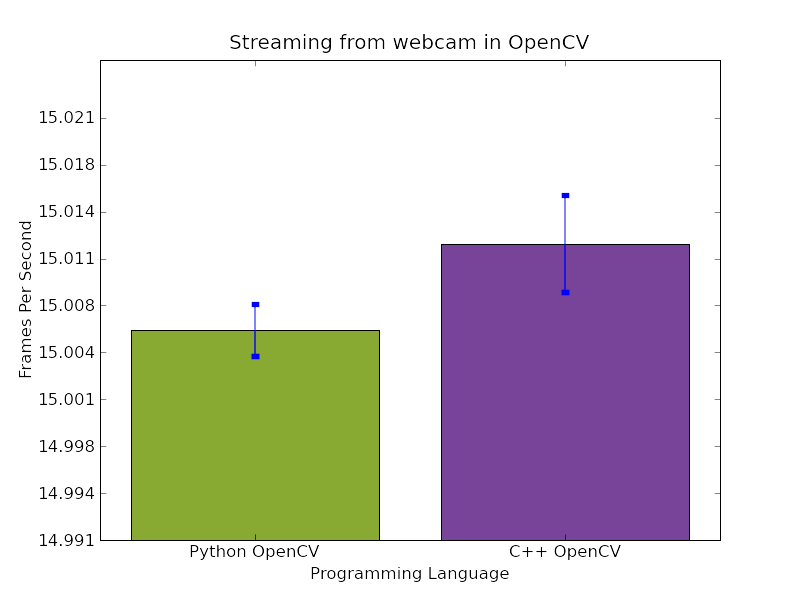
\includegraphics[width=0.8\columnwidth]{report_data/streaming_from_webcam_in_opencv}\caption{\label{fig:Streaming-comparison}Comparison of Python and C++ performance
using OpenCV for webcam capture and display.}

\end{figure}



\subsubsection{Comparison}

Figure \ref{fig:Streaming-comparison} shows performance results for
taking an image from a webcam and displaying the image with OpenCV.
The average frames per second were taken with 3 iterations, each averaging
the framerate over a 2 minute period. The error bars show standard
deviation of the sampled data. As Figure \ref{fig:Streaming-comparison}
shows, Python and C++ perform at very similar rates whilst carrying
out an I/O bound task. C++ having the expected result of a marginally
higher frame rate output than Python. The SciPy package does not currently
have a direct method for image capture.


\subsection{Image Blur}

One of the simplest operations in image processing is blurring an
image. This can be achieved in a few ways, the method looked at here
is by adding gaussian blur. Mathematically this is achieved by convolving
the image with a gaussian filter. Because of the separability of multidimensional
gaussian filters\cite{young1995recursive}, the convolution can be
applied in two ways; applying a 1 dimensional filter twice, once in
each direction; or secondly the image can be convolved with a 2-dimensional
gaussian filter created by the product of two 1 dimensional filters.
Equation \ref{eq:1D Gaussian Filter} shows the gaussian function
for obtaining the filter is in one dimension\cite{SS01}. \begin{equation}
G\left(x\right)=\frac{1}{\sqrt{2\pi}\sigma}e^{-\frac{x^{2}}{2\sigma^{2}}}\label{eq:1D Gaussian Filter}\end{equation}
\begin{equation}
G\left(x,y\right)=\frac{1}{\sqrt{2\pi}\sigma^{2}}e^{-\frac{x^{2}+y^{2}}{2\sigma^{2}}}\label{eq:2D Gaussian Filter}\end{equation}
Equation \ref{eq:2D Gaussian Filter} shows the 2 dimensional case\cite{SS01}.
OpenCV includes a gaussian filter that can be applied to an image
by calling the \emph{\noun{cvSmooth}} function and passing the desired
window size. SciPy has a n-dimensional Gaussian filter that acts on
a NumPy array. Both libraries use the 1 dimensional case, as it requires
less calculations.

In all implementations of this test an object oriented approach is
used, this ensures timing consistency between tests, and reduces code
duplication. 

The algorithms differ in that in order for the SciPy implementation
to work, the image data must be converted into NumPy arrays before
blurring. To continue using the OpenCV camera capture, the image data
must be converted into NumPy arrays. This has been achieved by creating
and using a Python decorator which converts before and after calling
a Python function using NumPy. A (640x480) RGB image takes less than
2ms to convert either way on the testing platform used throughout
this report. Also to ensure the same level of filtering is carried
out in all tests, the filter parameters need converted to be compatible
with OpenCV's \noun{cvSmooth} defaults\cite{bradski2008learning}.


\subsubsection{Comparison}

As expected the images produced by this are blurred as shown in Figure
\ref{fig:Gaussian-Output-Images}. For qualitative comparison a static
input image was used. What is not immediately obvious without further
investigation is how similar the results are. The OpenCV images produced
by C++ and Python are exactly the same pixel for pixel, this is expected
because the same library is doing the filtering. More interesting
is Figure \ref{fig:Difference-of-each} which shows that the SciPy
and OpenCV Python code doing the filtering produces very similar but
slightly different results. %
\begin{figure}
\begin{centering}
\subfloat[C++]{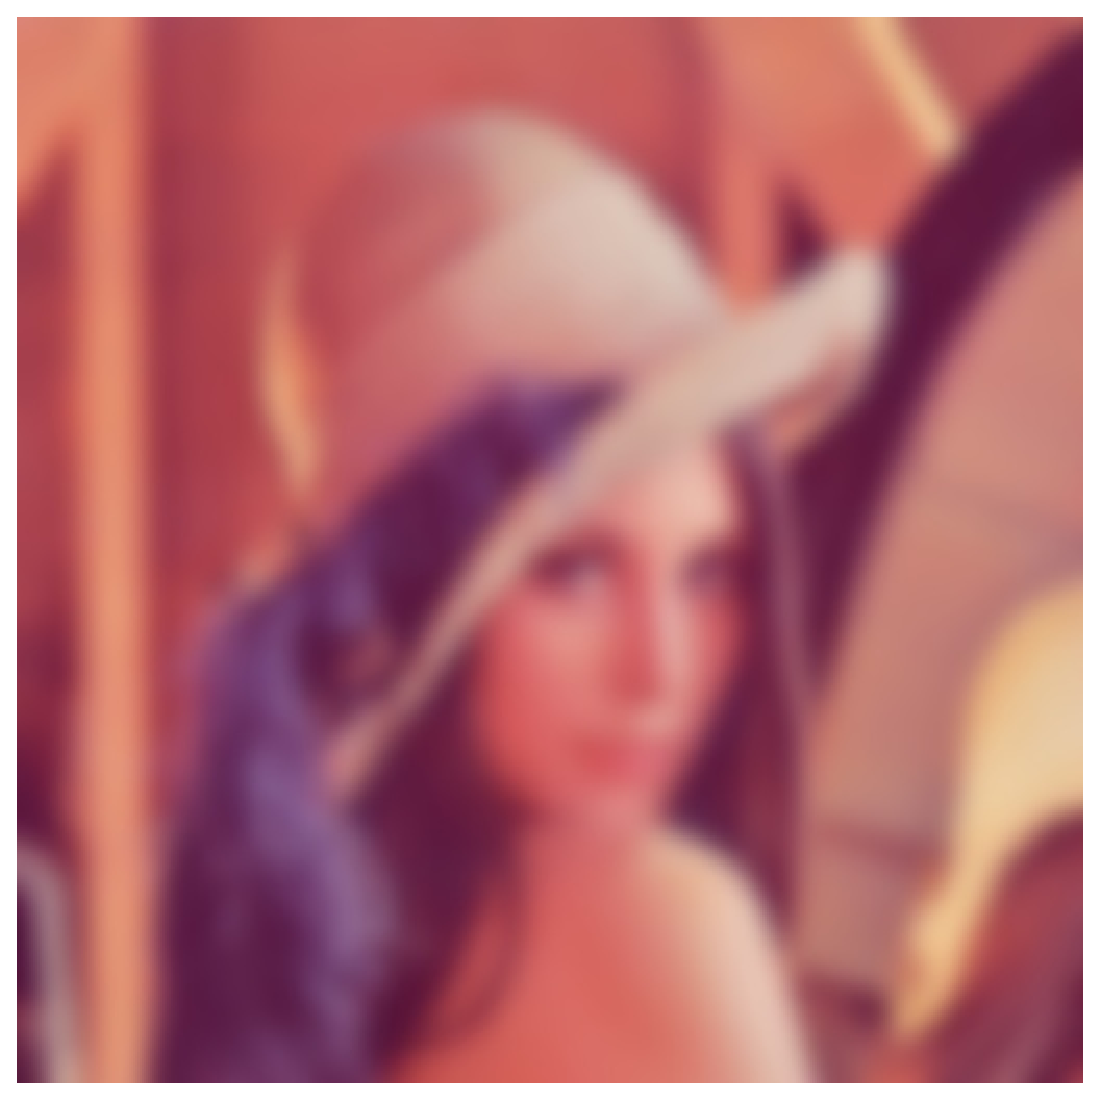
\includegraphics[width=0.3\columnwidth]{report_data/blurred_imag_cpp_opencv_gaussian}

}\subfloat[Python OpenCV]{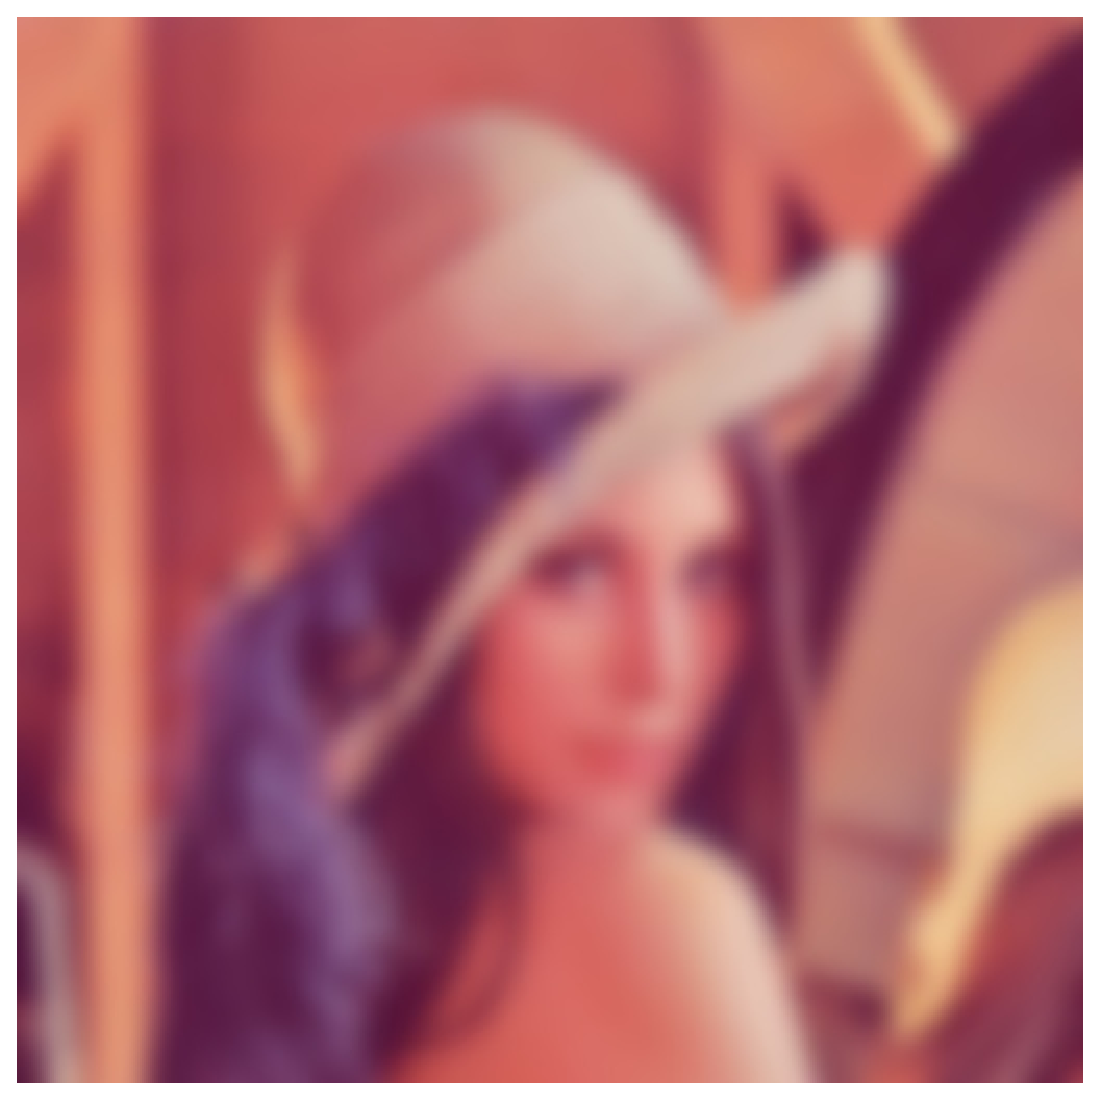
\includegraphics[width=0.3\columnwidth]{report_data/blurred_imag_python_opencv_gaussian}

}\subfloat[Python SciPy]{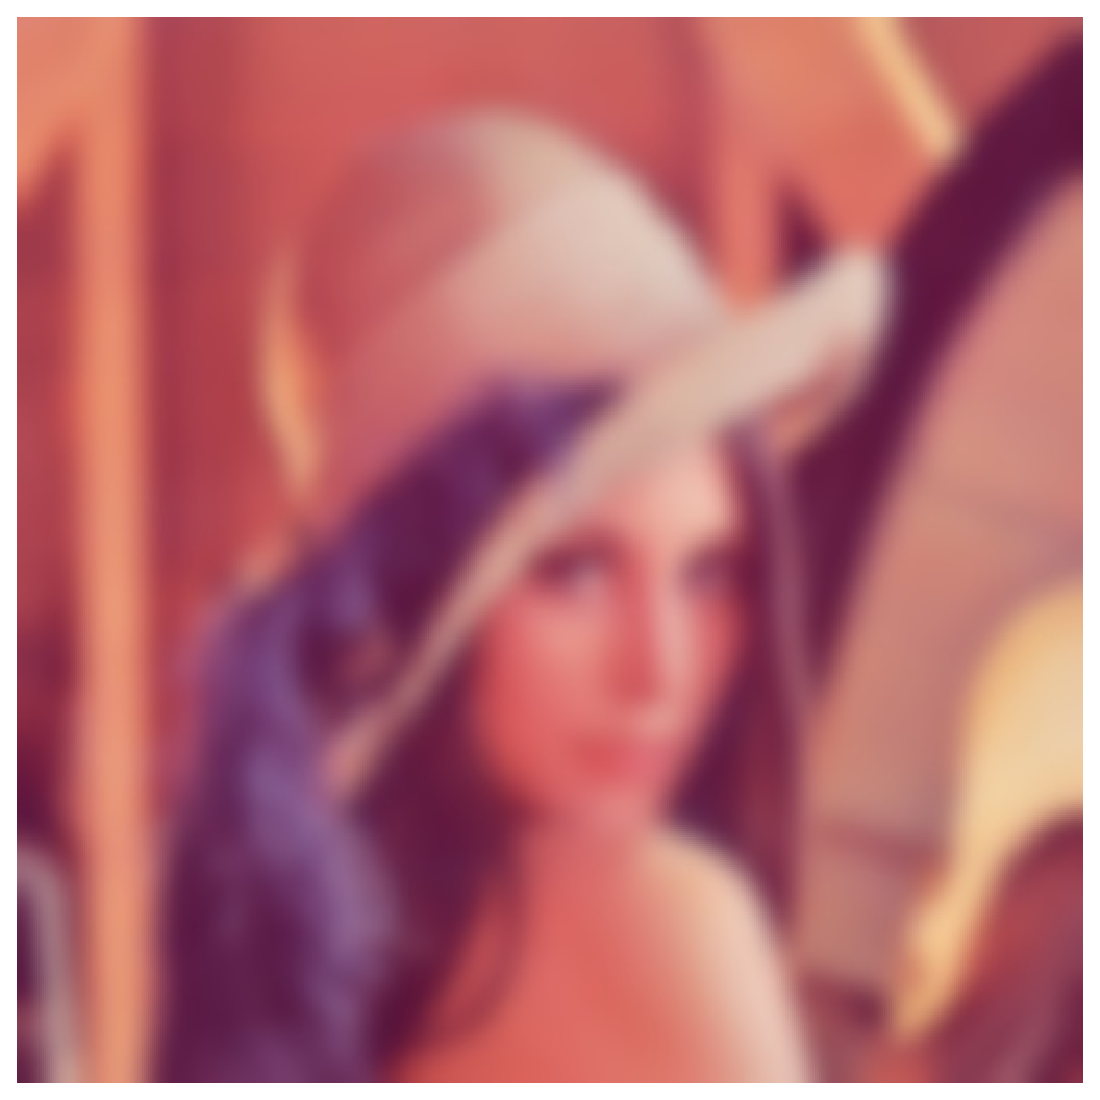
\includegraphics[width=0.3\columnwidth]{report_data/blurred_imag_python_scipy_gaussian}

}
\par\end{centering}

\caption{\label{fig:Gaussian-Output-Images}Output Images from Gaussian Blur
Examples}

\end{figure}
%
\begin{figure}[h]
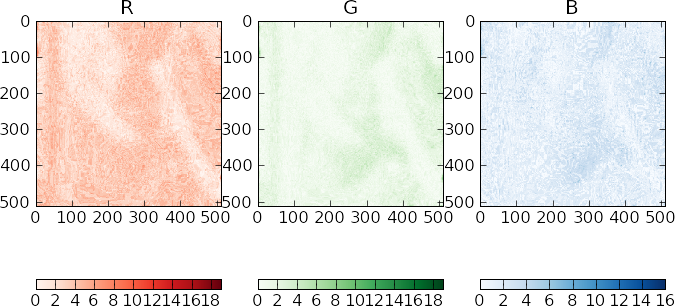
\includegraphics[width=0.95\columnwidth]{report_data/gaussian_diffs}

\caption{\label{fig:Difference-of-each}Difference of each channel after gaussian
blur in OpenCV and SciPy. Note full scale is 255, Pixel for pixel
difference image stats: maximum intensity difference = 20, average
difference = 2.1, std dev = 1.4}

\end{figure}


This could be caused by a difference in the implementation of the
gaussian kernel approximations. Since SciPy uses the sigma parameter,
the filter is created by a direct sampling of the gaussian function.
OpenCV on the other hand, uses the size of the filter, this is a good
indication it probably uses the pascal triangle as a good approximation
for the Gaussian kernel\cite{ben1991image}.The graph in Figure \ref{fig:Difference-of-each}
shows a 3 way sub plot of a single image. This graph was created interactively
using the Python plotting package Matplotlib from IPython acting directly
on the data from OpenCV. With just two lines of Python code, which
can be put anywhere in a computer vision program, we can pause execution
and drop into a live interactive shell with full plotting capabilities.
{}``\emph{from IPython.Shell import IPShellEmbed}'' and {}``\emph{IPShellEmbed()()}''
This means that as developers, to debug a misbehaving program, we
can just jump right into the middle of a deeply nested loop, introspect
all variables, plot any signal or image, call any function, and accurately
time the execution of any function. This is massively in favor of
using Python.

%
\begin{figure}[H]
\begin{centering}
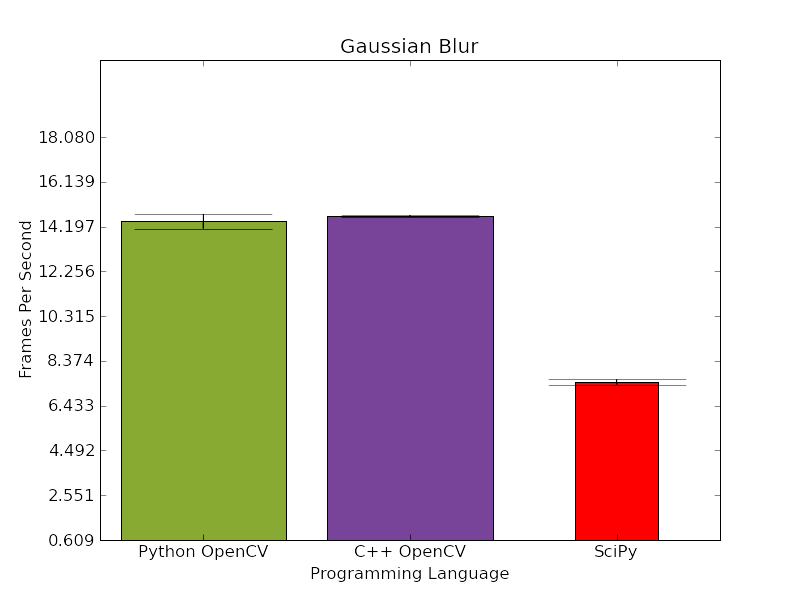
\includegraphics[width=0.8\columnwidth]{report_data/gaussian_blur}
\par\end{centering}

\caption{\label{fig:performance-gaussian}OpenCV performance carrying out Gaussian
Blur}



\end{figure}



\subsection{Background subtraction}

A common task in security surveillance, human interaction, and CV
in general is to detect movement in a video. This is done in its simplest
form by a comparison of one frame to another previous frame\cite{gao2006robust}.
If there is more than a threshold of difference, something changed.
The response is shown in Figure \ref{fig:Adding-a-single} after adding
a cellphone to the scene for the \noun{Python\_CV} implementation. 

%
\begin{figure}[h]
\subfloat[\label{fig:Adding-a-single}Adding item]{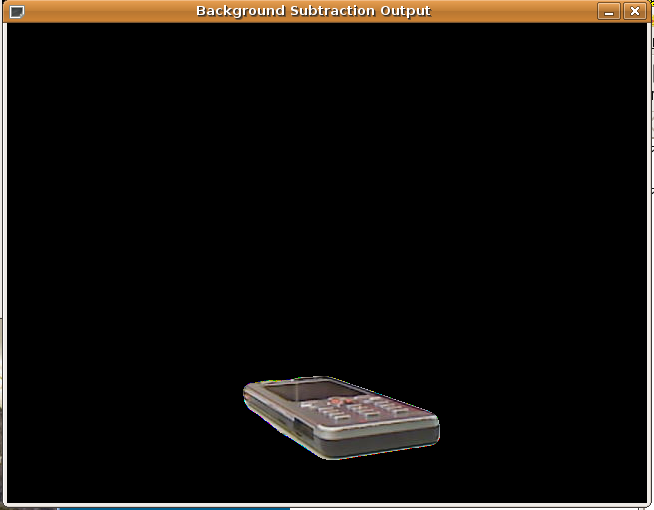
\includegraphics[width=0.3\columnwidth]{report_data/background_python_add_item}}\subfloat[\label{fig:Adding-another-item,}minor problems]{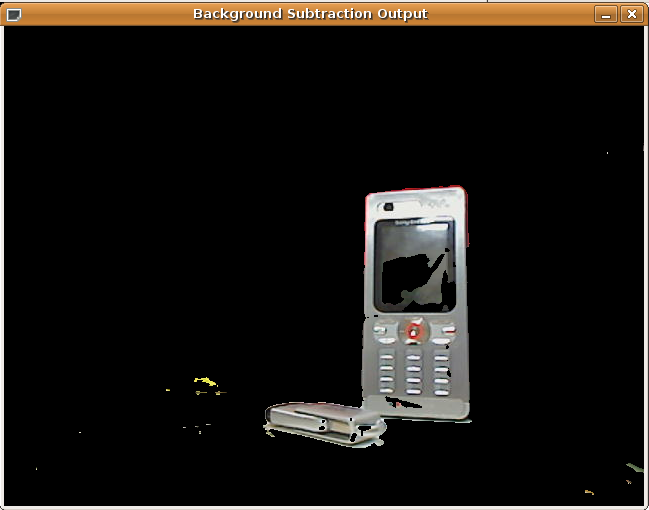
\includegraphics[width=0.3\columnwidth]{report_data/background_python_add_more_items}

}\subfloat[\label{fig:remove-laptop}Addition and removal]{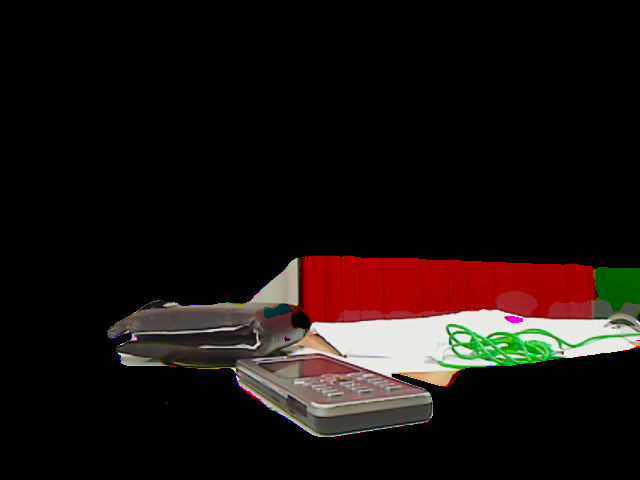
\includegraphics[width=0.3\columnwidth]{report_data/background_python_add_remove_item}

}

\caption{\label{fig:background-Adding-and-removing}Background subtraction
response to adding and removing items from a scene.}

\end{figure}
%
\begin{figure}
\subfloat[before]{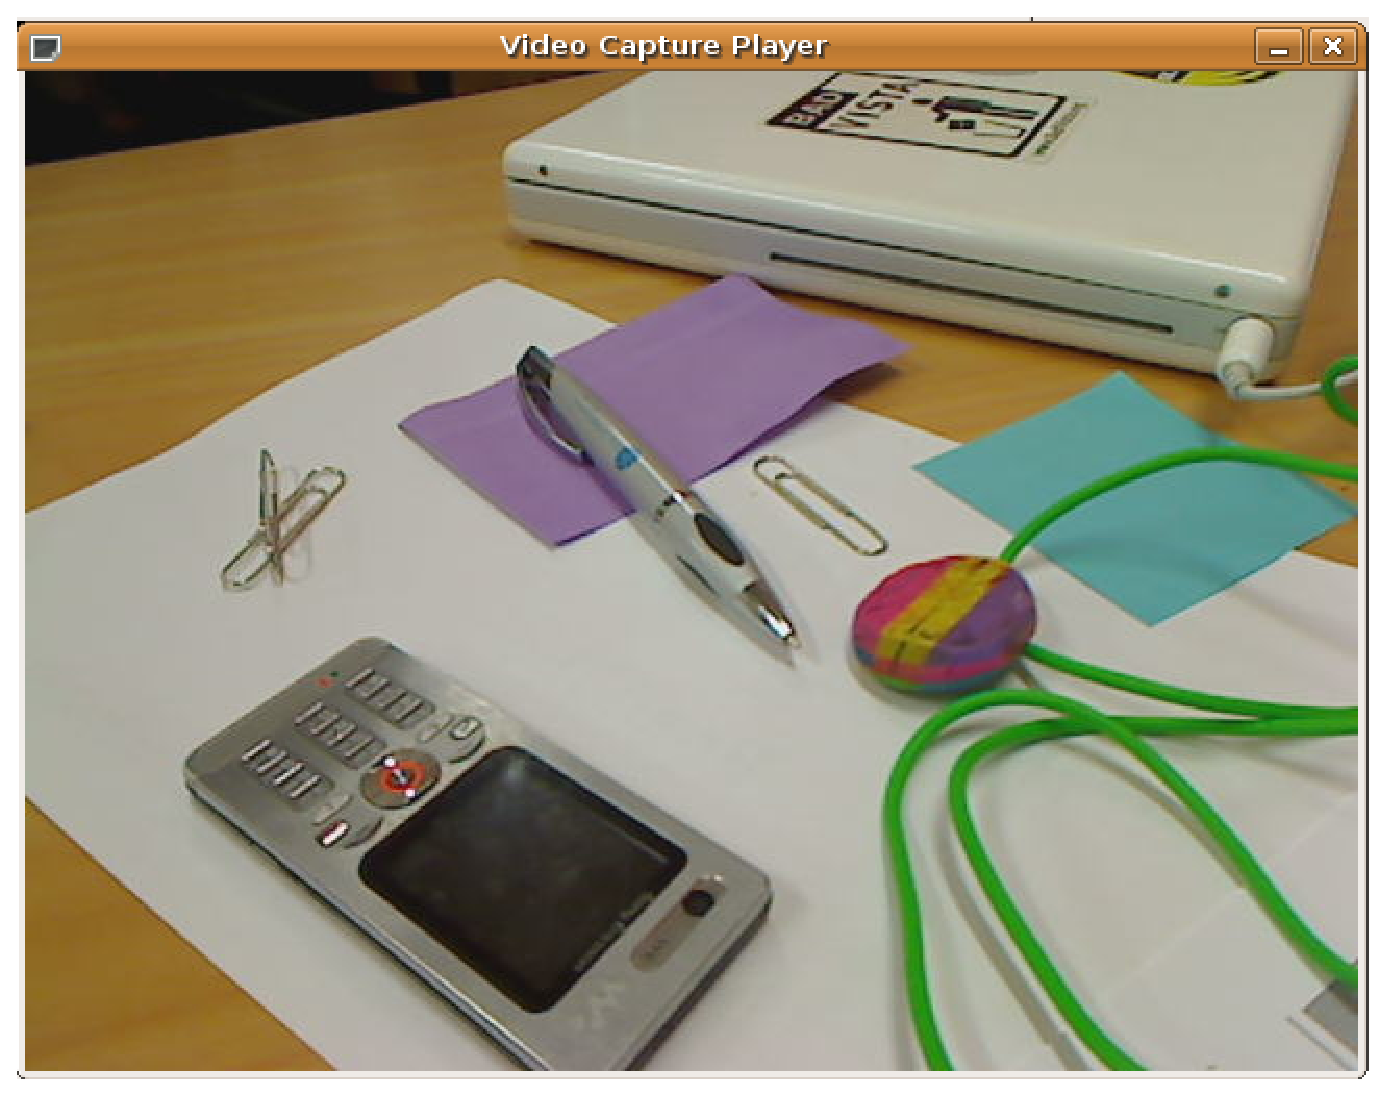
\includegraphics[width=0.3\columnwidth]{report_data/background_python_before}

}\subfloat[program output]{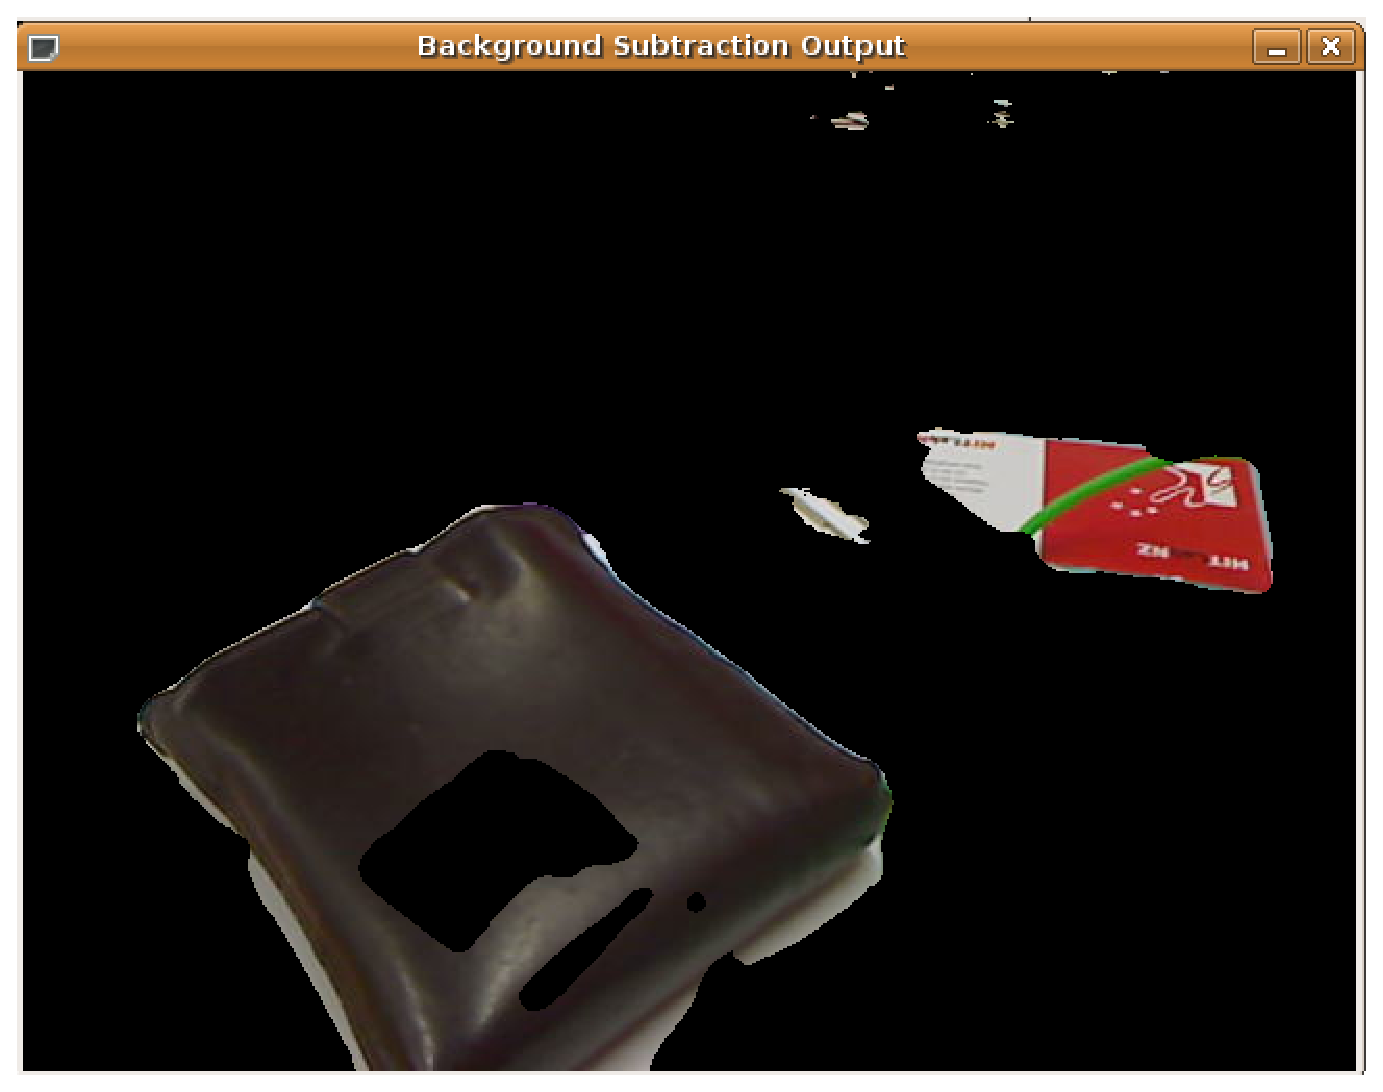
\includegraphics[width=0.3\columnwidth]{report_data/background_python_add_items_complicated}

}\subfloat[after]{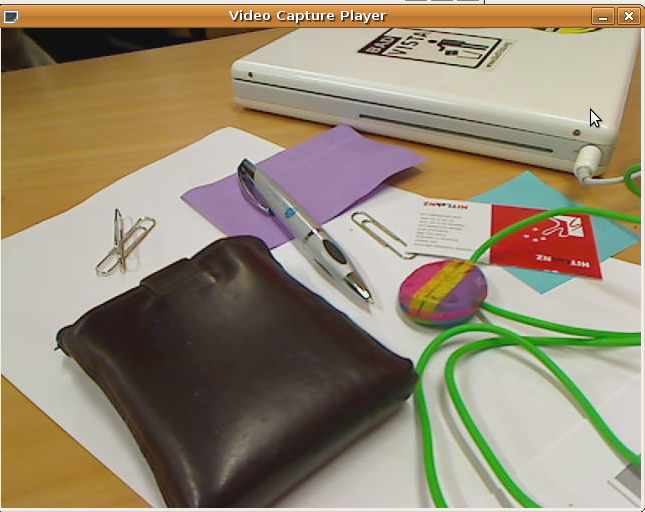
\includegraphics[width=0.3\columnwidth]{report_data/background_python_after}

}

\caption{\label{fig:back-Proces-clutter}Background subtraction response on
a cluttered scene where a cellphone is switched for a wallet and a
contact card is added.}

\end{figure}
 While creating this program, we found IPython particularly helpful,
it allows for interactive, in place trialing, timing and plotting
as shown in algorithm \ref{alg:Interactive,-inplace-timing}.

%
\begin{algorithm}
\noindent In {[}1{]}: from opencv import cv

\noindent In {[}2{]}: cv.cvAnd(diffImage,image, temp)

\noindent In {[}3{]}: timeit cv.cvAnd(diffImage,image, temp)

\noindent 1000 loops, best of 3: 229 \textmu{}s per loop

\noindent In {[}4{]}: from pylab import imshow, show

\noindent In {[}5{]}: imshow(temp) 

\noindent Out{[}5{]}: <AxesImage object at 0x42489d0>

\noindent In {[}6{]}: show()

\caption{\label{alg:Interactive,-inplace-timing}Using IPython, the interactive
shell can be used from deep inside a nested loop in a running program.
In place timing and plotting with access to local variables and functions
like this example speeds up development time.}

\end{algorithm}



\subsection{Feature Point Detection}

Many methods in computer vision for identifying the contents of an
image relies on extracting \emph{interesting} features. An interesting
feature point could be corners of intersecting lines, a line ending,
or any isolated point where local image regions have a high degree
of variation in all directions\cite{harris1988combined}. The features
must be found algorithmically and have a well-defined position. The
repeatability of choosing the same points under differing conditions
is a measure of how good an interesting feature algorithm is. The
corner detection algorithm works by locating points where the surroundings
have edges in more than one direction. According to \cite{Sol09}
the Harris \& Stephens algorithm is in short: 
\begin{quote}
A matrix W is created from the outer product of the image gradient,
this matrix is averaged over a region and then a corner response function
is defined as the ratio of the determinant to the trace of W.
\end{quote}
A threshold is then applied to this corner response image to pick
the most likely candidates and then these points are plotted. An example
usage of the algorithm is in the Lucas\textendash{}Kanade Optical
Flow Method where it can be used to select good feature points\cite{beauchemin1995computation}
for tracking movement.

%
\begin{figure}[h]
\begin{centering}
\subfloat[\label{fig:harris_scipy_static}SciPy]{\begin{centering}
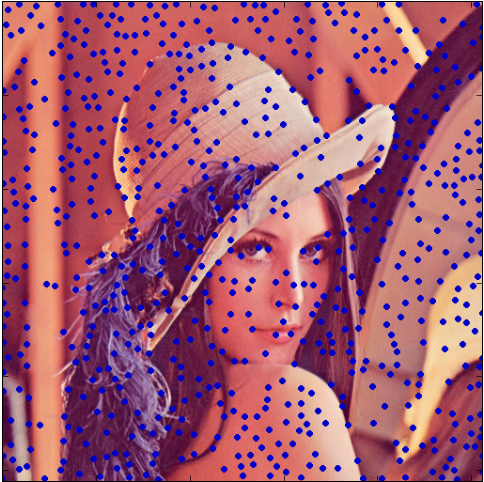
\includegraphics[width=0.45\columnwidth]{harris_scipy_static}
\par\end{centering}

}\subfloat[OpenCV]{\centering{}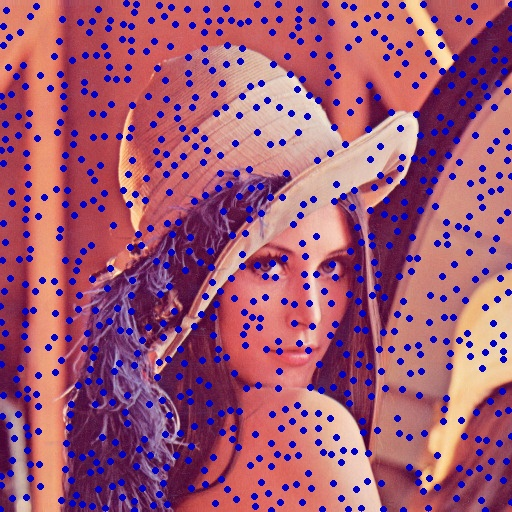
\includegraphics[width=0.45\columnwidth]{harris_response_lena_opencv}}
\par\end{centering}

\caption{\label{fig:harris_compare_static}Running the Harris \& Stephens feature
detection algorithm on the Lena test image.}

\end{figure}
%
\begin{figure}[h]
\begin{centering}
\subfloat[\label{fig:harris_webcam_scipy}SciPy (\textasciitilde{}4fps)]{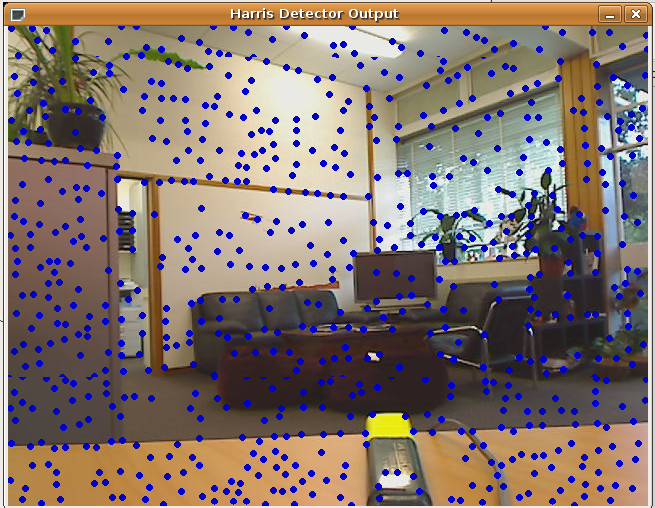
\includegraphics[width=0.45\columnwidth]{report_data/feature_detect/scipy_harris}

}\subfloat[OpenCV (\textasciitilde{}9fps)]{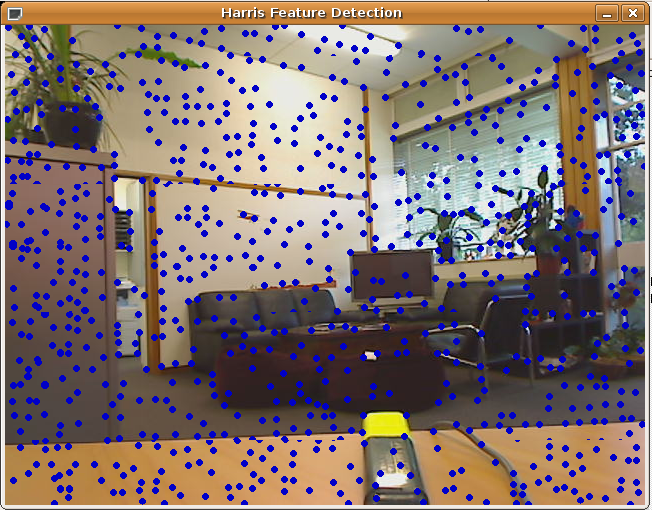
\includegraphics[width=0.45\columnwidth]{report_data/feature_detect/opencv_harris}

}
\par\end{centering}

\caption{\label{fig:harris_compare_webcam}Feature detection running on webcam
stream}

\end{figure}


We took and modified an existing implementation in SciPy by \cite{Sol09}
which produced Figures \ref{fig:harris_webcam_scipy} \& \ref{fig:harris_scipy_static}.
The algorithm was timed by executing it on Lena 300 times per sample:

\begin{center}
\begin{tabular}{|c|c|c|}
\hline 
Sample: & Mean & Std\tabularnewline
\hline
\hline 
SciPy & 191.5 ms & 0.87 ms\tabularnewline
\hline 
OpenCV & 65.7 ms & 1.27 ms\tabularnewline
\hline
\end{tabular}
\par\end{center}

The same concept but in a different implementation is shown in Figure
\ref{fig:harris_compare_webcam} for OpenCV. An aperture size of 3
pixels was used when computing the harris response, the authors did
note that with a larger aperture SciPy seemed to slow down more than
OpenCV. To reduce differences between the algorithms the threshold
filtering and display of the corner response is done just in OpenCV,
the SciPy implementaiton therefore has to convert the data before
this stage. Another limitation is that the OpenCV response in C++
is not implemented here.


\subsection{Face Detection}

Face detection is the task of locating any number of faces in an image,
this is a specific case of general object detection. Before locating
an object, one must be able to describe it. Many object detection
algorithms use a classifier which is a collection of feature patterns
made by scanning a database of images with known content. Figure \ref{fig:OpenCV-Face-Detection}
shows the output from our tests running under different conditions
when using the face Haar-cascade classifier that comes with OpenCV.
The method gave a mean framerate of 7.16 \textpm{} 0.02 Hz. The detection
process itself gave very consistent timings of 107 \textpm{} 1 ms.
The detection method used has limitations as shown in Figures \ref{fig:Obscured-opencv-face}
and \ref{fig:Angled-opencv-face}. But in ideal conditions, with good
lighting and un-obscured faces directly facing the camera the algorithm
produces very good results. In this example we did not find corresponding
high level functionality in SciPy, so no performance comparison is
possible.

%
\begin{figure}[h]
\subfloat[Single face in frame]{\begin{centering}
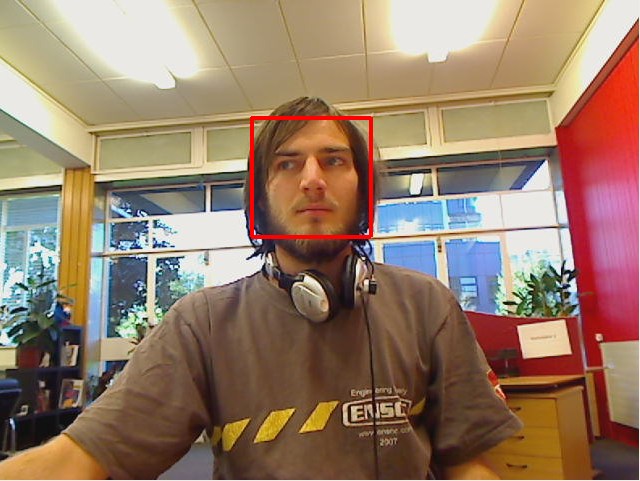
\includegraphics[width=0.45\columnwidth]{report_data/face_detect_one}
\par\end{centering}



}\subfloat[\label{fig:Obscured-opencv-face}Obscured face in frame]{\begin{centering}
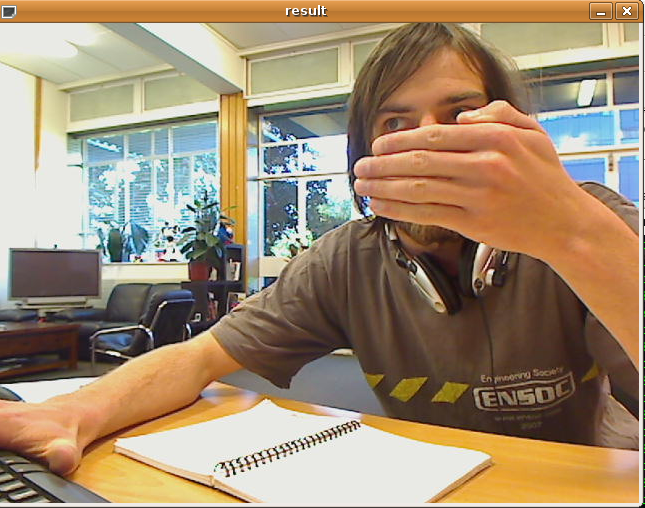
\includegraphics[width=0.45\columnwidth]{report_data/face_detect_obscure}
\par\end{centering}



}

\subfloat[Multiple faces]{\begin{centering}
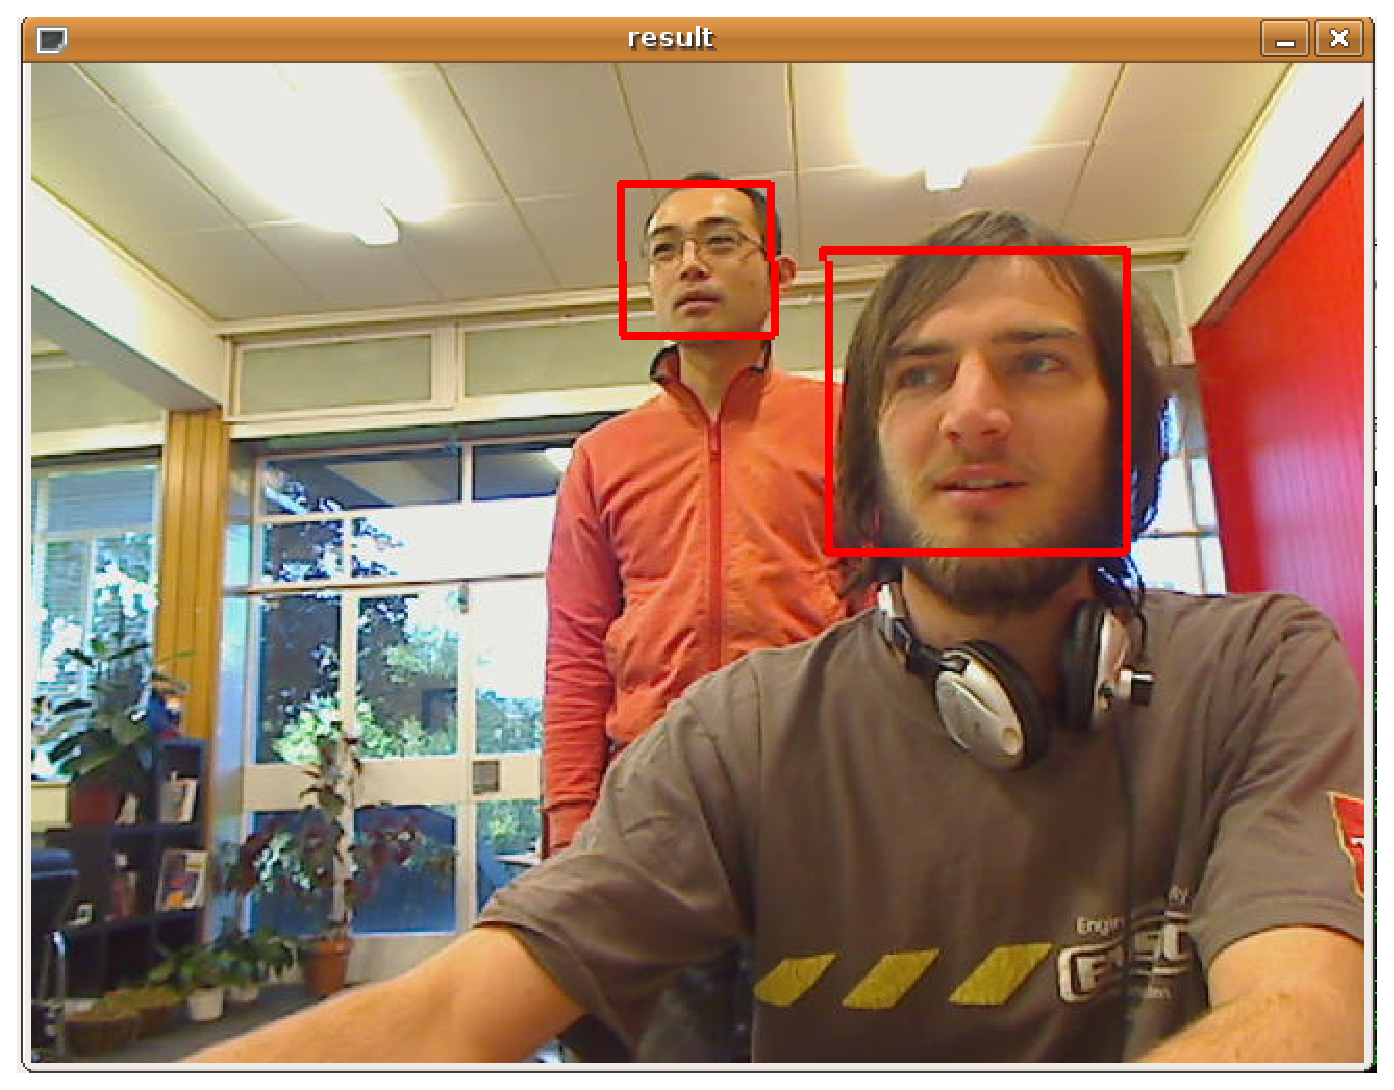
\includegraphics[width=0.45\columnwidth]{report_data/face_detect_two}
\par\end{centering}



}\subfloat[\label{fig:Angled-opencv-face}Rotated face]{\begin{centering}
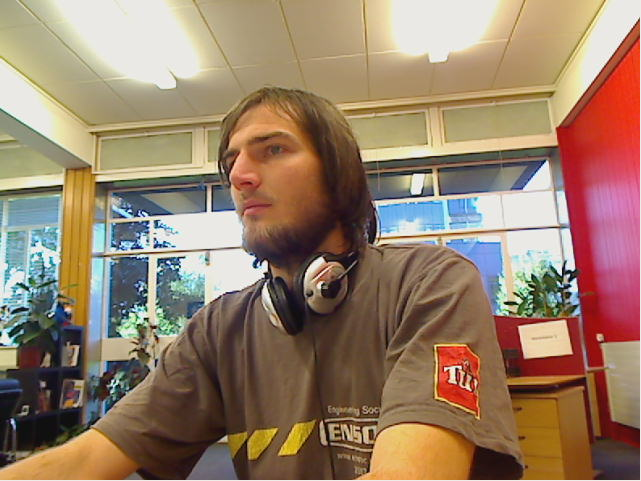
\includegraphics[width=0.45\columnwidth]{report_data/face_detect_sideways}
\par\end{centering}



}

\caption{\label{fig:OpenCV-Face-Detection}OpenCV Face Detection}

\end{figure}


%
\begin{figure}
\begin{centering}
\subfloat[detecting face objects]{\begin{centering}
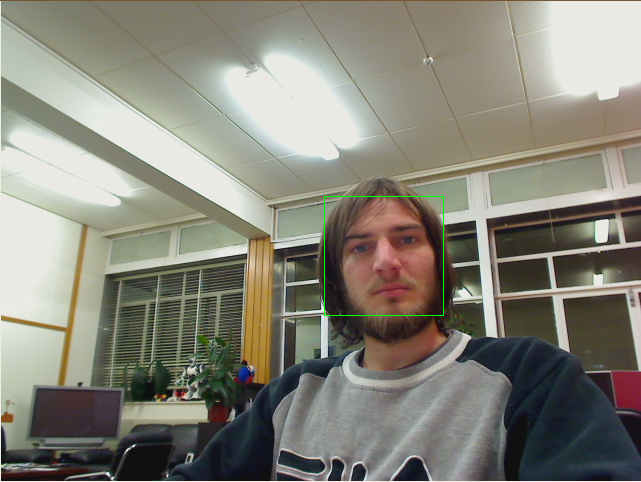
\includegraphics[width=0.4\columnwidth]{report_data/pygame-eye-locate}
\par\end{centering}



}\subfloat[\label{fig:edge-filtering-face}edge filtering and face detection]{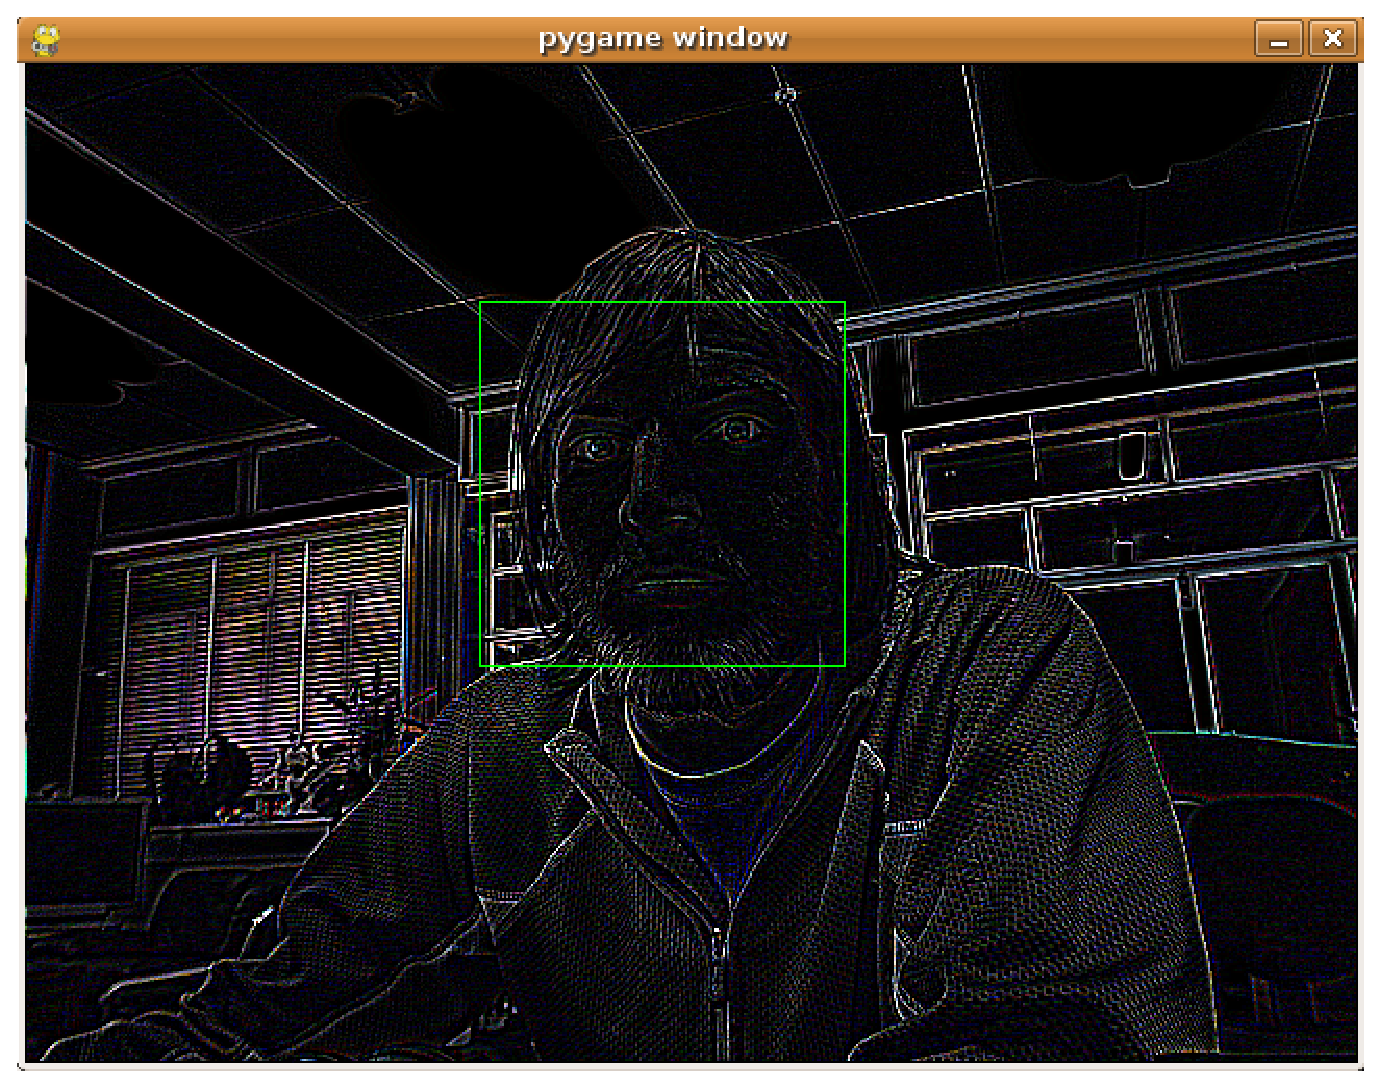
\includegraphics[width=0.4\columnwidth]{report_data/pygame-face-edge}



}
\par\end{centering}

\caption{\label{fig:Pygame-object}Pygame can be used to capture and display
the webcam, while OpenCV does the processing.}



\end{figure}


Figure \ref{fig:Pygame-object} shows an alternative setup; using
the Pygame camera module for image capture, OpenCV for the object
detection and Pygame surfaces for the box rendering and display. Python
really shows its strengths as a glue language here, as the different
libraries are easily used in conjunction with each other. The benefits
from this can be huge, it is very easy for a developer to incorporate
different computer vision tools, even with very limited knowledge
of computer vision. We found that calling OpenCV from a Python wrapper
was only slightly slower in general than natively using the library. 


\section{Qualitative Comparison}

In getting these quantitative results we noticed that the Python implementations
were shorter, easier to create, easier to debug, and easier to test.
Having the use of an interactive interpreter, to come to a solution
prototype and being able to use these prototypes in the final product
is a big argument in favor of using Python. 

The documentation in both SciPy and OpenCV was found to be complete,
but not as extensive as for a professional package like Matlab. Support
for these open source packages is almost entirely reliant on experienced
members of the community responding to requests on message boards
or mailing lists. When one of the authors asked a question regarding
the gaussian image filtering function to the SciPy mailing list it
spurred not only an immediate response pointing out the solution to
the direct query but also a discussion on finite approximations to
gaussian kernels, how OpenCV might do it differently, and a user even
went as far as to test and propose a new IIR filter implementaition
for SciPy that scales better with kernel size than the existing implementations.
This kind of support is quite common in the open source world, where
a package like SciPy prides itself on its very rigorous and open tests. 

For the scholar of Computer Vision research we find that using Python
can help in trying out new algorithms, very quickly. The breadth of
the additional libraries available and the ease of integrating make
new and novel solutions quickly realizable. 

For those newer to computer vision, we recommend Python for many reasons,
mainly it is much more forgiving than C or C++, it can be used interactively
so you can happily make 10 mistakes in a row, without having to recompile
for each attempted fix. 

A major limitation of using Python would be when the application is
being developed for special or embedded hardware or when the best
possible performance is required.


\section{Related Works}

A feature of SciPy that has previously gone unmentioned, is the Weave
module for in-lining C and C++ code. This can easily produce code
100x\cite{ramachandran-performance} faster than pure Python. \cite{cai2005performance}
showed that for parallel programming, mixed language solutions exhibit
the same performance gains as native language solutions from moving
to parallel solutions. Another related area of research is the performance
of Python itself. One such project was the Psyco just in time compiler
for Python\cite{rigo2004representation}, unfortunaly Psyco only works
on Python 2.6.X and on x86 machines. The developer is currently working
on the performance of PyPy, a compliant, flexible and fast implementation
of the Python Language. Google is currently midway through their Unladen
Swallow project which aims to speed up Python by leveraging the Low
Level Virtual Machine (LLVM). All of these projects make Python a
safe bet for the future of scientific computing and specifically the
often performance capped computer vision domain.
\begin{itemize}
\item Performance speed ups with NumPy\cite{cai2005performance}
\item GPUCV\cite{farrugia2006gpucv}\cite{allusse2008gpucv}
\item Pyro - \cite{blank2003pyro} introduced Pyro, a robotics simulation
environment
\item Pygame - a game making package for Python, aimed at new programmers.
It has a camera module and is able to do basic computer vision tasks,
or call on any other Python library e.g. SciPy/NumPy. http://pygame.org
\item Pycam - All test and example code from this project. http://pycam.googlecode.com
\end{itemize}

\subsection*{Acknowledgments}

Thanks to all the developers that invest their own valuable time to
work on open source projects OpenCV, Python and SciPy.


\section{Appendix}

\bibliographystyle{ieeetr}
\bibliography{report_data/database}

\end{document}
